%\documentclass{article}
\documentclass{article}
\usepackage{tikz}
\usepackage{tikz-dependency}
\usepackage{multirow}
\usepackage{caption} 
\captionsetup[table]{skip=10pt}
\usepackage{array}
\newcolumntype{C}[1]{>{\centering\let\newline\\\arraybackslash\hspace{0pt}}m{#1}}
\usepackage[T1]{fontenc}


\begin{document}

\begin{table}[ht] 
   \begin{tabular}{  c | l  r } \hline 
%      catena &  type & \hspace{1cm}HI & Mixed\hspace{2.8cm} HF \hspace{1cm} \\
        type & \multicolumn{2}{l}{\hspace{0.5cm} Head-initial\hspace{2cm} Mixed\hspace{2.5cm} Head-final} \\
   \hline
 relative clause & \parbox[c]{14em}{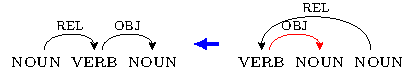
\includegraphics[width=5cm, height=1.4cm]{relative/REL_HI.pdf}} &\parbox[c]{14em}{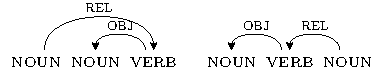
\includegraphics[width=5cm, height=1.4cm]{relative/REL_HF.pdf}} \\
 complement clause & \parbox[c]{14em}{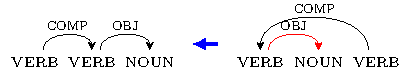
\includegraphics[width=5cm, height=1.4cm]{complement/COMP_HI.pdf}} &\parbox[c]{14em}{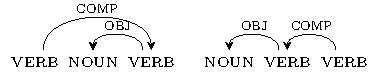
\includegraphics[width=5cm, height=1.4cm]{complement/COMP_HF.pdf}} \\
genitive & \parbox[c]{14em}{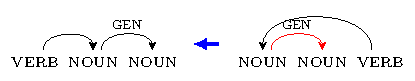
\includegraphics[width=5cm, height=1.4cm]{genitive/Gen_HI.pdf}} &\parbox[c]{14em}{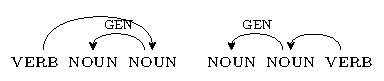
\includegraphics[width=5cm, height=1.4cm]{genitive/Gen_HF.pdf}} \\
%adjective/adverb & \parbox[c]{14em}{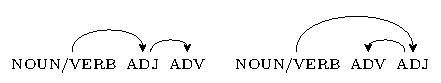
\includegraphics[width=5cm, height=1.4cm]{adjective_adverbs/ADJ_ADV_HI.pdf}} &\parbox[c]{14em}{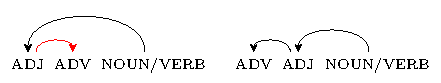
\includegraphics[width=5cm, height=1.4cm]{adjective_adverbs/ADJ_ADV_HF.pdf}} \\
    \hline
  \end{tabular}
\end{table}

\end{document}